
\chapter{Разработка программы решения теоретико-графовой задачи на
  языке программирования C++}

В следующем разделе я описываю выполнение второго этапа расчетной
работы на примере задачи поиска одного из минимальных путей в
неориентированном графе. Для понимания руководства студент должен
обладать следующими знаниями:

\begin{itemize}
\item базовыми знаниями по языку C++;
\item базовыми знаниями по работе с STL-контейнерами std::set,
  std::map, std::list, std::pair.
\end{itemize}

\section{Задание}

На этом этапе выполнения расчетной работы вам необходимо будет
разработать программу с использованием библиотеки моделирования
sc-памяти, которая бы решала вашу теоретико-графовую задачу на основе
формализации предметной области, проведенной на предыдущем этапе. Сам
алгоритм вы уже исследовали в прошлом семестре, но сейчас надо будет
не просто реализовать какой-то алгоритма, а адаптировать его к
графодинамическому способу обработки информации. Это значит, что вся
информация, необходимая для работы вашего алгоритма, должна храниться
в sc-памяти и там же и обрабатываться. В качестве примера
<<неудобства>>, которое вам может принести такое требование, я могу
привести невозможность использования привычной матрицы
смежности/инцидентности.  Поэтому для прохождения этого этапа вам
придется взглянуть на алгоритм, решающий выбранную задачу, под другим
углом.

В качестве тестов для написанной программы необходимо использовать
тестовые примеры, которые вы сделали в ходе предыдущего этапа
расчетной работы.

\section{Установка и настройка рабочей среды}

Для начала мы установим и настроим рабочую среду для программирования
с использованием программной модели sc-памяти и запустим
программу-пример, которая использует эту модель. Всё описанное в этой
главе программное обеспечение можно найти как в интернете, так и на
кафедральном сервере info. На сервере info весь материал и всё
программное обеспечение располагается по следующему пути:
\begin{verbatim}
\\Info\StudInfo\~Методическое обеспечение кафедры\~Учебные курсы\2 курс\ППвИС\@Расчётная работа
\end{verbatim}

Во-первых, нам необходимо скачать и установить программный модуль
sc-core, который представляет собой ядро для обработки
sc-текстов. Инсталлятор для этого модуля можно взять в следующих
местах:

\begin{itemize}
\item скачать из папки
  \href{http://sourceforge.net/projects/ostis/files/kpm/}{kpm}
  sc-core-0.2.5-win32.exe (работает с MS Visual Studio 9)
\item скачать по следующему пути sc-core-0.2.5.exe (работает с MS
  Visual Studio 9):
\begin{verbatim}
\\Info\StudInfo\~Методическое обеспечение кафедры\~Учебные курсы\2 курс\ППвИС\@Расчётная работа\sc-core-0.2.5.exe
\end{verbatim}
\item скачать по следующему пути sc-core-0.2.5-vc10-bin-win32.exe
  (работает с MS Visual Studio 10):
\begin{verbatim}
\\Info\StudInfo\~Методическое обеспечение кафедры\~Учебные курсы\2 курс\ППвИС\@Расчётная работа\sc-core-0.2.5-vc10-bin-win32.exe
\end{verbatim}
\end{itemize}

После того, как вы скачали инсталлятор, запустите его. Желательно
устанавливать sc-core так, чтобы полный путь к установленной папке не
содержал пробелов в именах директорий. При установке необходимо
выбрать опцию, которая добавит директорию исполняемых файлов sc-core в
переменную среды окружения \verb+PATH+ (см. рис.~\ref{fig:Add_sc_core_to_path}).

\begin{figure}[h]
  \centering
  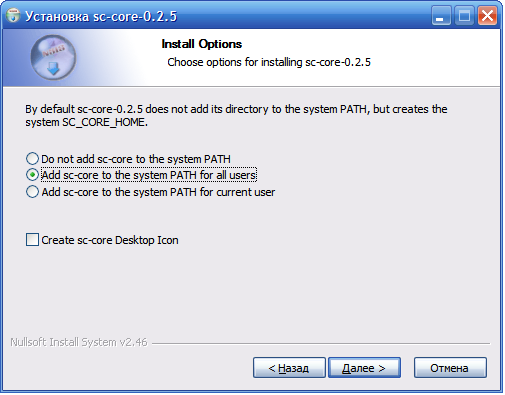
\includegraphics[scale=0.7]{4/setup/Add_sc_core_to_path}
  \caption{Добавление директории исполняемых файлов sc-core в
    системную переменную PATH для всех пользователей}
  \label{fig:Add_sc_core_to_path}
\end{figure}
 
Мной была выбрана установка sc-core в папку
\verb+"c:\\sc-core"+. После установки данного модуля были изменены
следующие переменные среды окружения:
\begin{itemize}
\item \verb+SC_CORE_HOME+, которая теперь имеет значение
  \verb+"c:\sc-core"+
\item \verb+PATH+, к которой была добавлена директория
  \verb+"c:\sc-core\bin"+
\end{itemize}

В дальнейшем для указания пути к директории sc-core я буду
использовать значение переменной среды окружения \verb+SC_CORE_HOME+.

Для сборки примера нам еще будет необходима программа
CMake. Необходимо скачать установочный файл для версии не ниже 2.6.2
или взять инсталлятор из папки расчетной работы на сервере info. Как и
при установке sc-core, при установке CMake необходимо выбрать опцию,
которая добавит директорию исполняемых файлов в переменную среды
окружения \verb+PATH+ (см. рис.~\ref{Add_cmake_to_path}).
 
\begin{figure}[h]
  \centering
  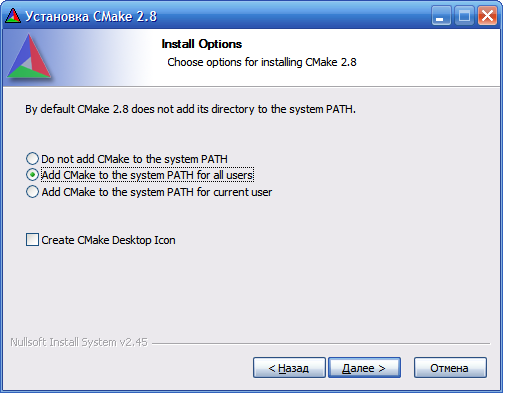
\includegraphics[scale=0.7]{4/setup/Add_cmake_to_path}
  \caption{Добавление CMake в системную переменную PATH для всех
    пользователей}
  \label{fig:Add_cmake_to_path}
\end{figure}

С модулем sc-core версии 0.2.5 идет старая версия примера
использования библиотеки моделирования sc-памяти, поэтому я рекомендую
вам взять из папки на сервере info файл с именем
\verb+wave_find_path.cpp+ и скопировать его в приеденную ниже папку,
заменив существующий там файл с таким именем. После этого перейдем к
генерации проекта для примера:
\begin{verbatim}
%SC_CORE_HOME%\examples\wave_find_path
\end{verbatim}

Для генерации проекта примера воспользуемся консолью. Для запуска
консоли нажимаем клавиши \verb|Win + R|, в появившемся диалоге пишем cmd и
нажимаем Enter. На экране должно появиться следующее окно, как
показано на рисунке 2.3.

\begin{figure}[h]
  \centering
  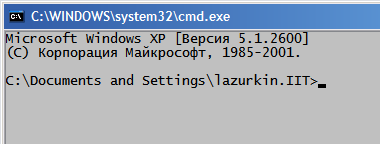
\includegraphics[scale=0.7]{4/setup/Run_console}
  \caption{Открытая консоль}
  \label{fig:Run_console}
\end{figure}

Переходим в директорию примера использования библиотеки моделирования
sc-памяти, используя команды:
\begin{verbatim}
c: 
cd %SC_CORE_HOME%\examples\wave_find_path
\end{verbatim}

%\begin{figure}[h]
%  \centering
%  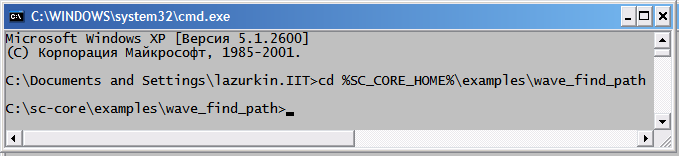
\includegraphics[scale=0.7]{4/setup/Cd_to_example_dir}
 % \caption{Переход в директорию примера wave\_find\_path}
  %\label{fig:Cd_to_example_dir}
%\end{figure}

% Если у вас Windows с русификацией, то могут возникнуть проблемы с запуском cmake. CMake будет сообщать о том, что он не может скопировать файлы "CMakeVSMacros1.vsmacros" и "CMakeVSMacros2.vsmacros" в "c:\Documents and Settings\lazurkin.IIT\Мои документы\Visual Studio 2008\Projects\VSMacros80\CMakeMacros" (это путь на моей файловой системе с моим именем пользователя, для вас он будет отличаться названием директории вашего пользователя). Эти файлы необходимо скопировать вручную. Для этого просто скопируйте содержимое "c:\Program Files\cmake2.8\share\cmake-2.8\Templates\" в "c:\Documents and Settings\lazurkin.IIT\Мои документы\Visual Studio 2008\Projects\VSMacros80\CMakeMacros" (этот путь для вас будет другой!!!). 

% При помощи следующей команды сгенерируем проект MS Visual Studio 9.0
% для сборки и запуска примера (в cmake есть генератор и для MS Visual
% Studio 10.0, просто введите команду cmake и на консоль будет выведен
% список всех доступных генераторов):

% cmake -G "Visual Studio 9 2008" .

 
% Рисунок 2.5 Генерация проекта для примера wave_find_path 
% Если у вас MS Visual Studio 2010, то можете попробовать команду:
% cmake .

% После корректной работы CMake в директории будет создан проект wave_find_path. Открываем его при помощи MS Visual Studio 9.0. Нажимаем правой кнопкой мыши на проекте wave_find_path в Solution Explorer и выбираем пункт меню "Set as StartUp Project". После этого название данного проекта будет выделено жирным цветом. Теперь можно запустить на исполнение пример wave_find_path (пример вывода на рисунке 2.6).
 
% Рисунок 2.6 Вывод работы программы-примера wave_find_path

%%% Local Variables: 
%%% mode: latex
%%% TeX-master: "main"
%%% End: 
